\documentclass{book}

\usepackage{graphicx}

\begin{document}
\title{Vitamins}
\author{Radu-Mihai Rotariu}
\maketitle

\tableofcontents
\chapter{Vitamin A}
\begin{figure}[h]
	\centering 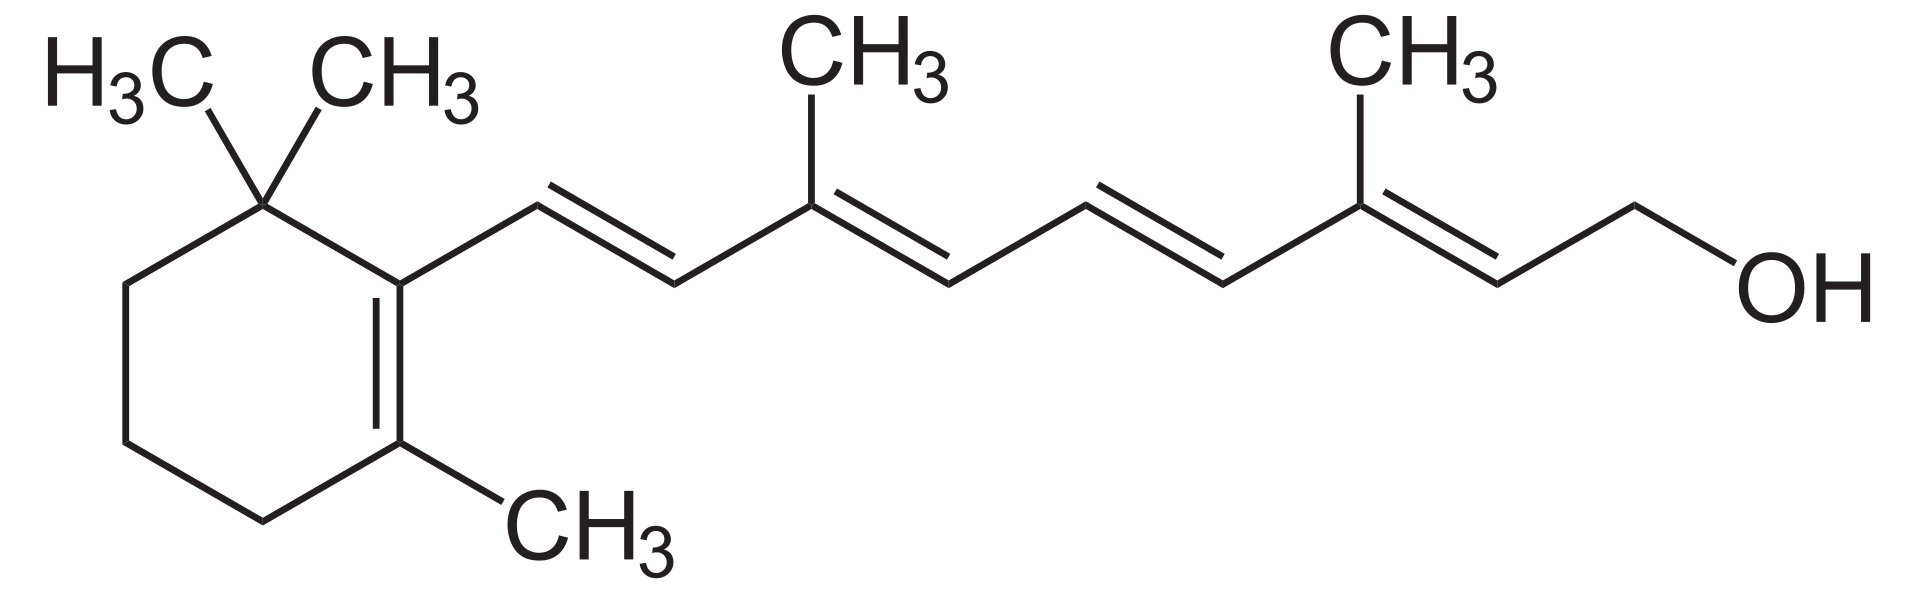
\includegraphics[width=\linewidth]{images/Vitamin_A_chemical_structure}
	\caption{Chemical structure of Vitamin A}
\end{figure}

\section{About}


\section{Measurement unit}


\section{Dietary recommendations}


\section{Sources}


\chapter{Vitamin B1}
\begin{figure}[h]
	\centering 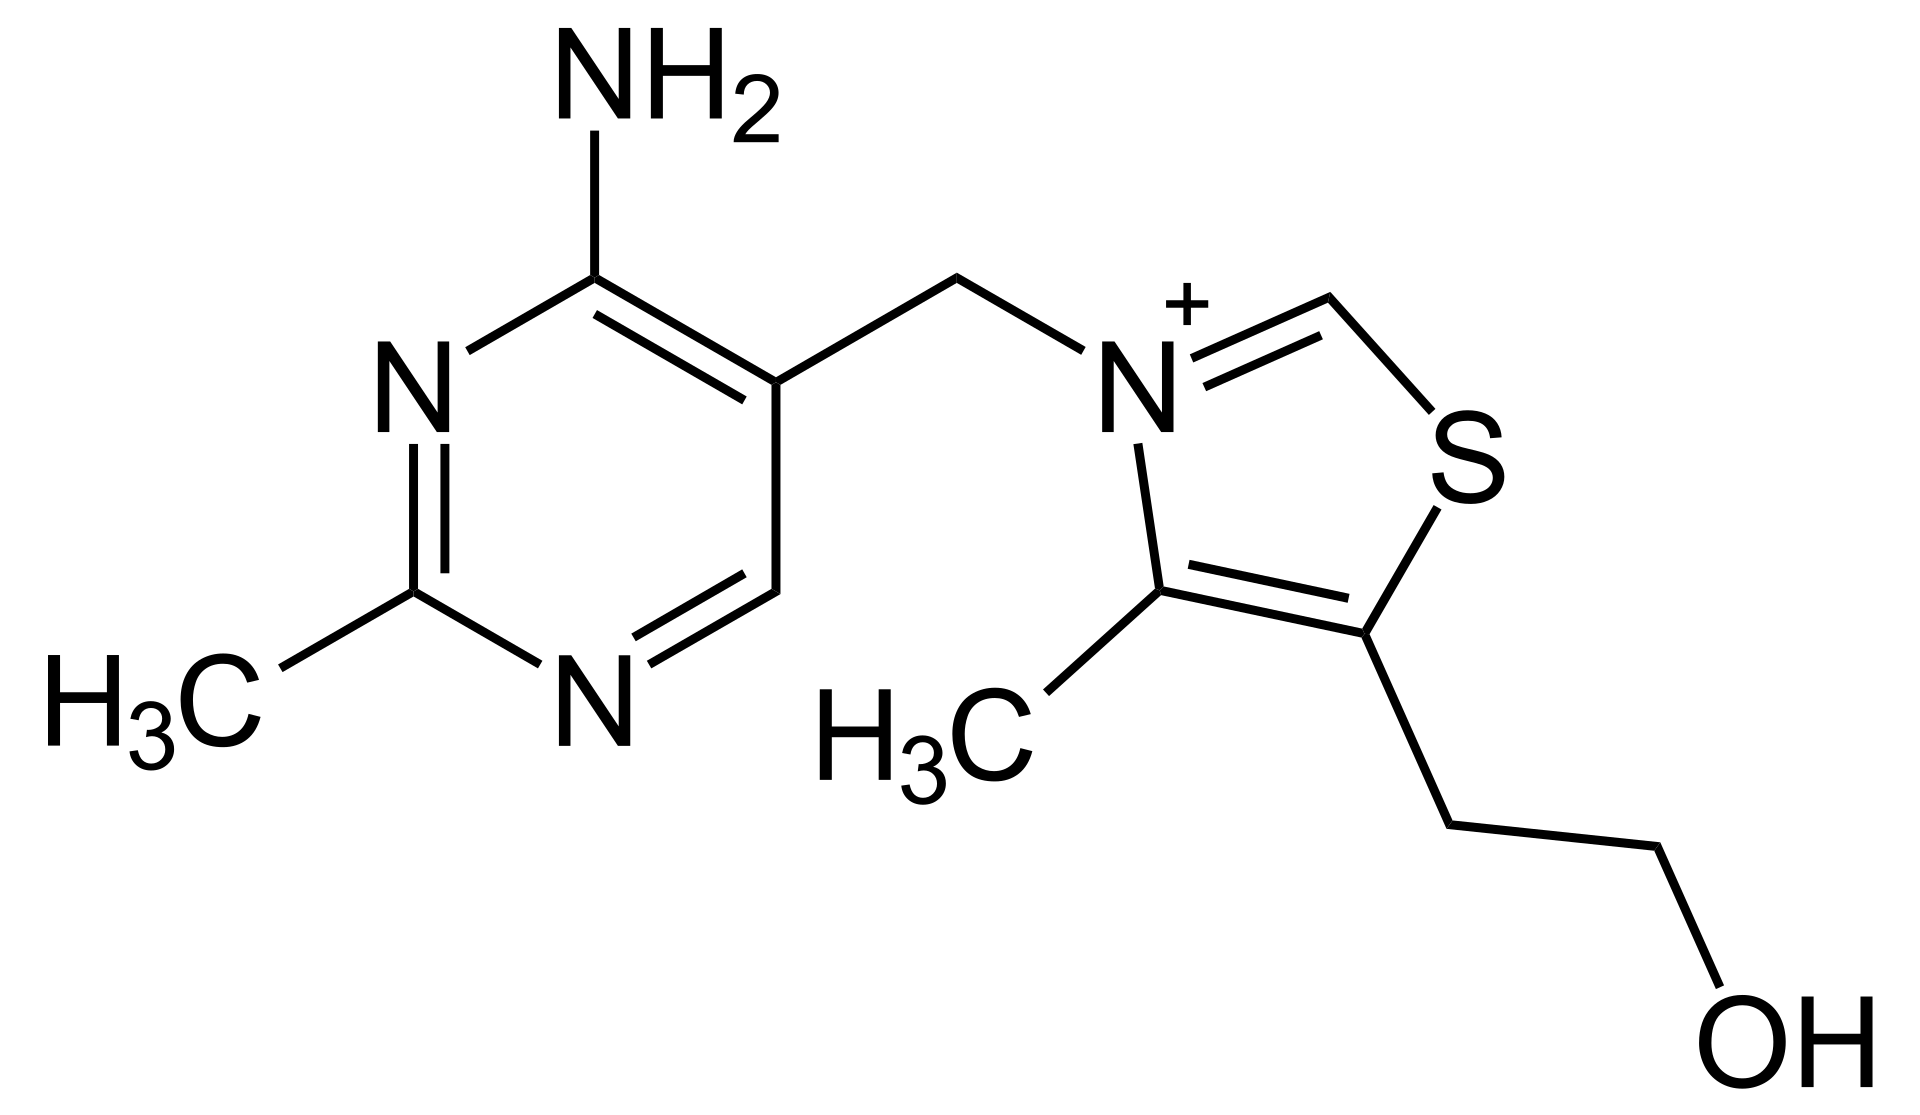
\includegraphics[width=0.75\linewidth]{images/Vitamin_B1_chemical_structure}
	\caption{Chemical structure of Vitamin B1}
\end{figure}

\section{About}


\section{Measurement unit}


\section{Dietary recommendations}


\section{Sources}


\chapter{Vitamin B2}
\begin{figure}[h]
	\centering 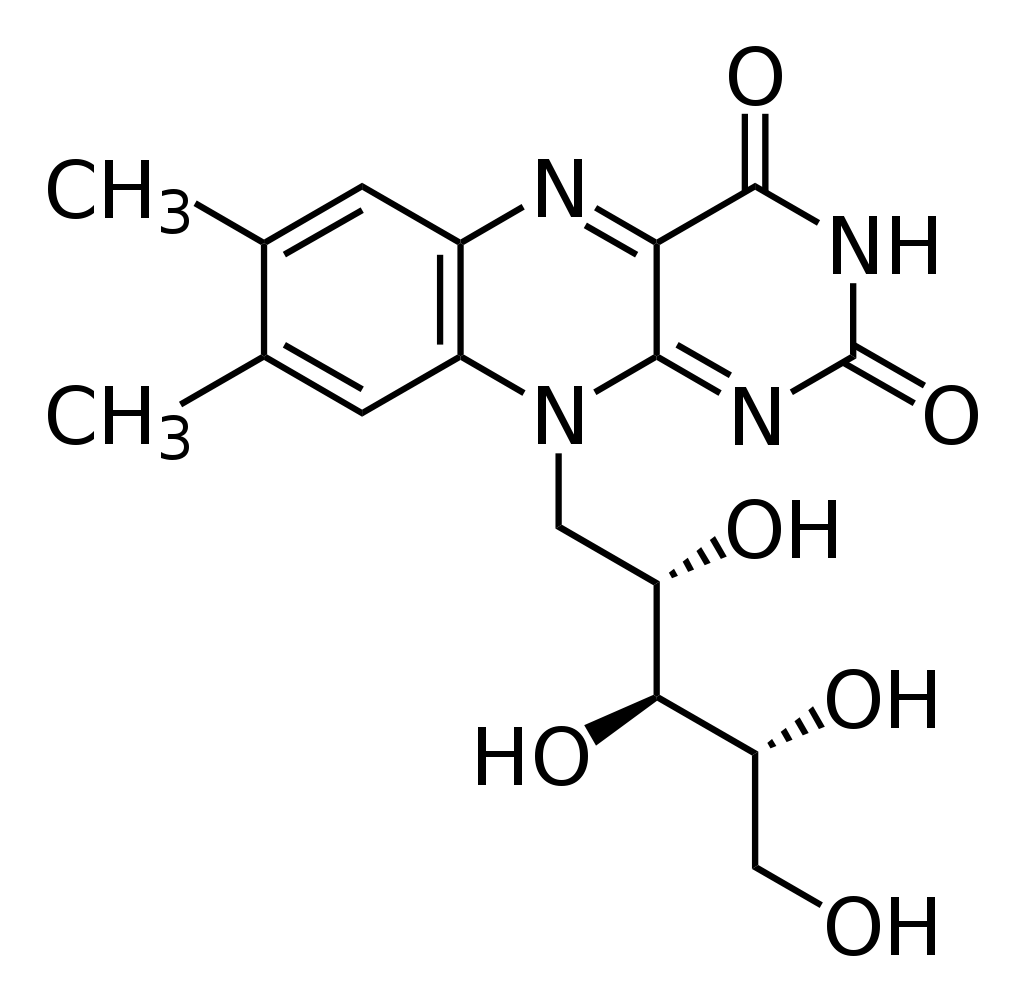
\includegraphics[width=0.75\linewidth]{images/Vitamin_B2_chemical_structure}
	\caption{Chemical structure of Vitamin B2}
\end{figure}

\section{About}


\section{Measurement unit}


\section{Dietary recommendations}


\section{Sources}


\chapter{Vitamin B3}
\begin{figure}[h]
	\centering 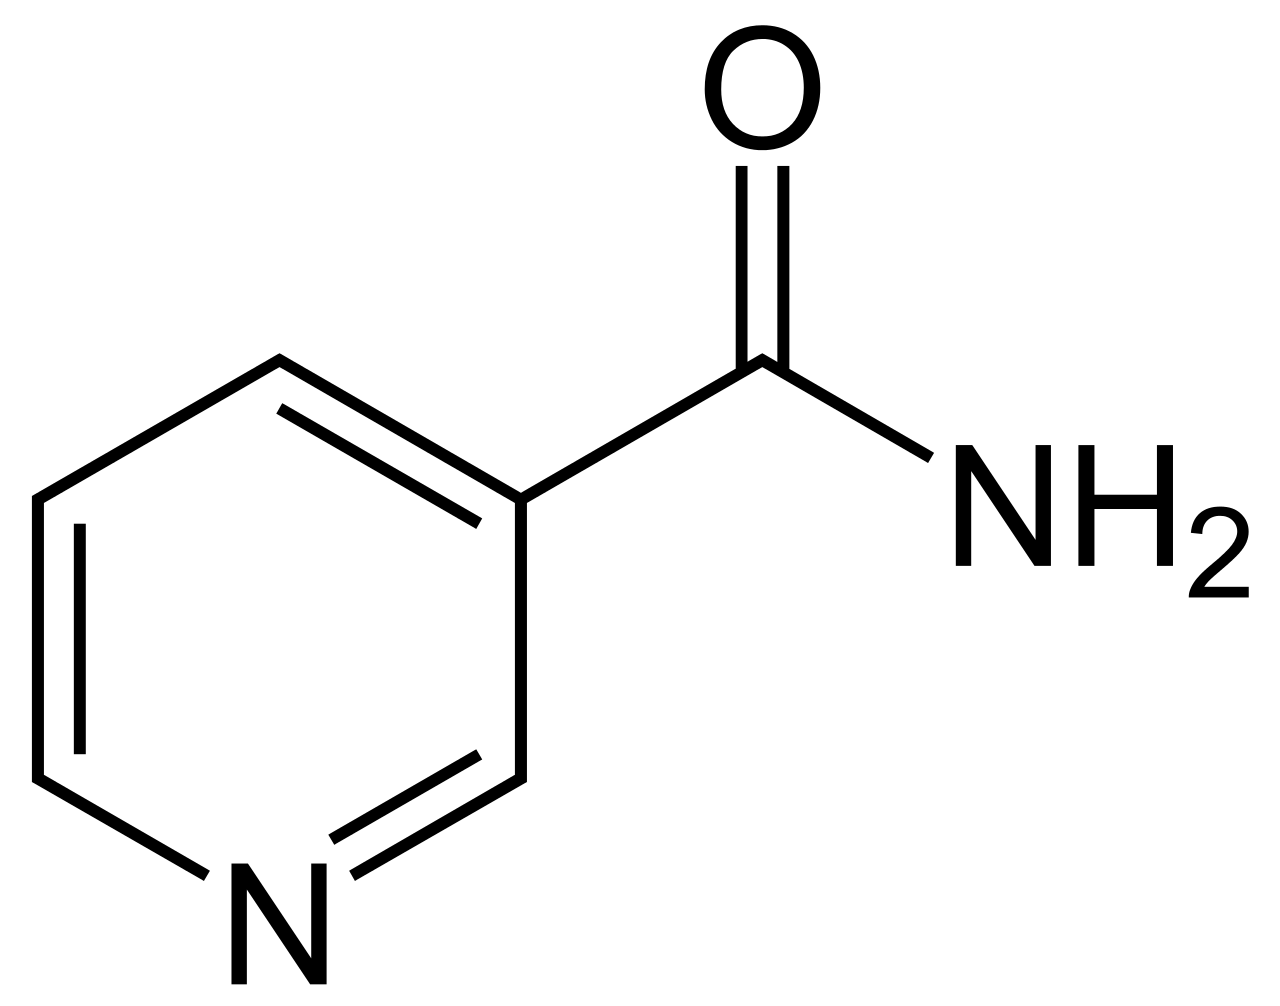
\includegraphics[width=0.75\linewidth]{images/Vitamin_B3_chemical_structure}
	\caption{Chemical structure of Vitamin B3}
\end{figure}

\section{About}


\section{Measurement unit}


\section{Dietary recommendations}


\section{Sources}


\chapter{Vitamin B5}
\begin{figure}[h]
	\centering 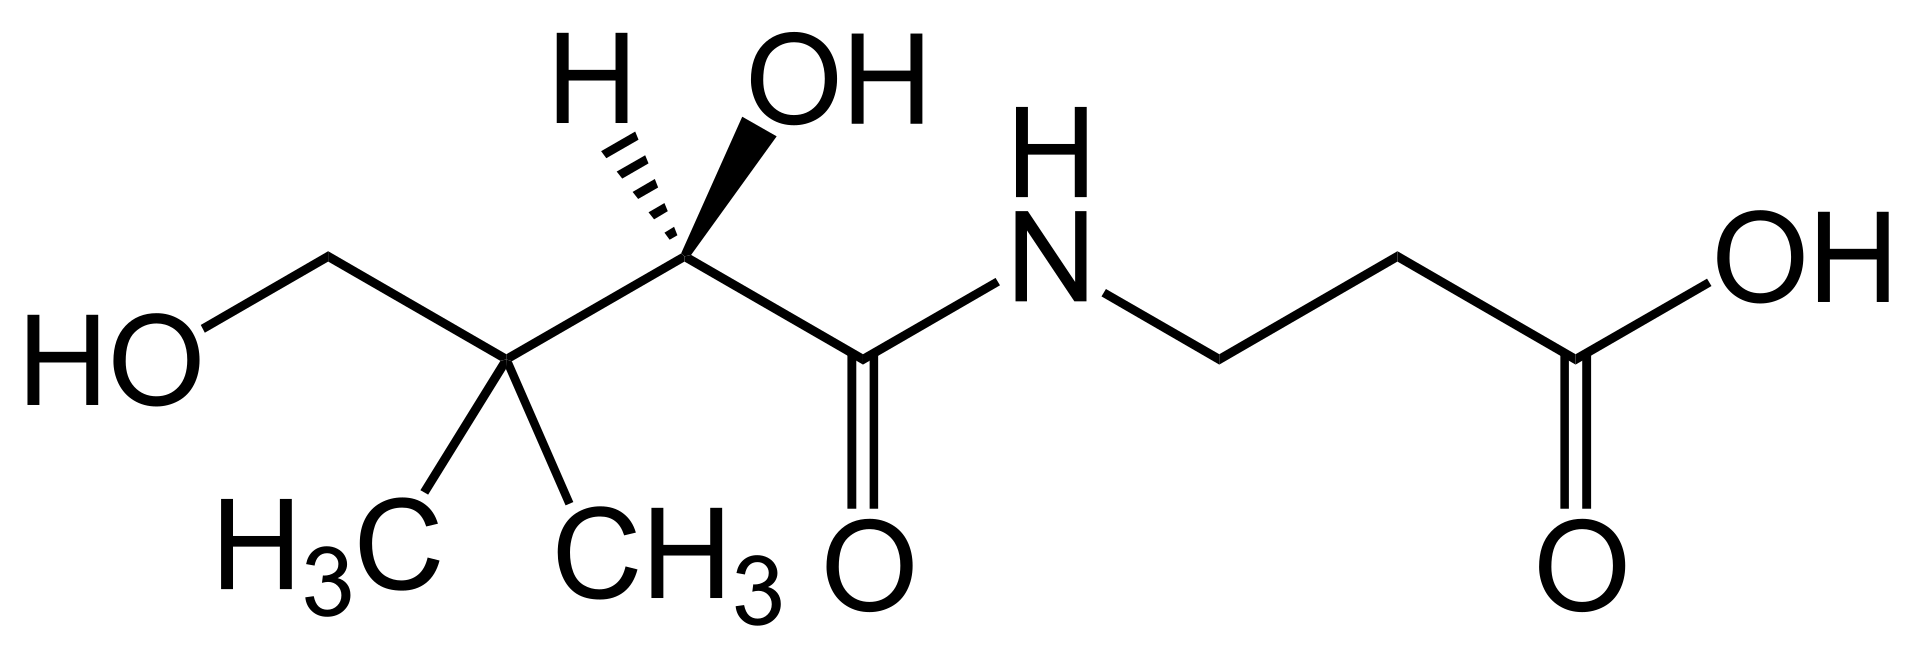
\includegraphics[width=0.75\linewidth]{images/Vitamin_B5_chemical_structure}
	\caption{Chemical structure of Vitamin B5}
\end{figure}

\section{About}


\section{Measurement unit}


\section{Dietary recommendations}


\section{Sources}


\chapter{Vitamin B6}
\begin{figure}[h]
	\centering 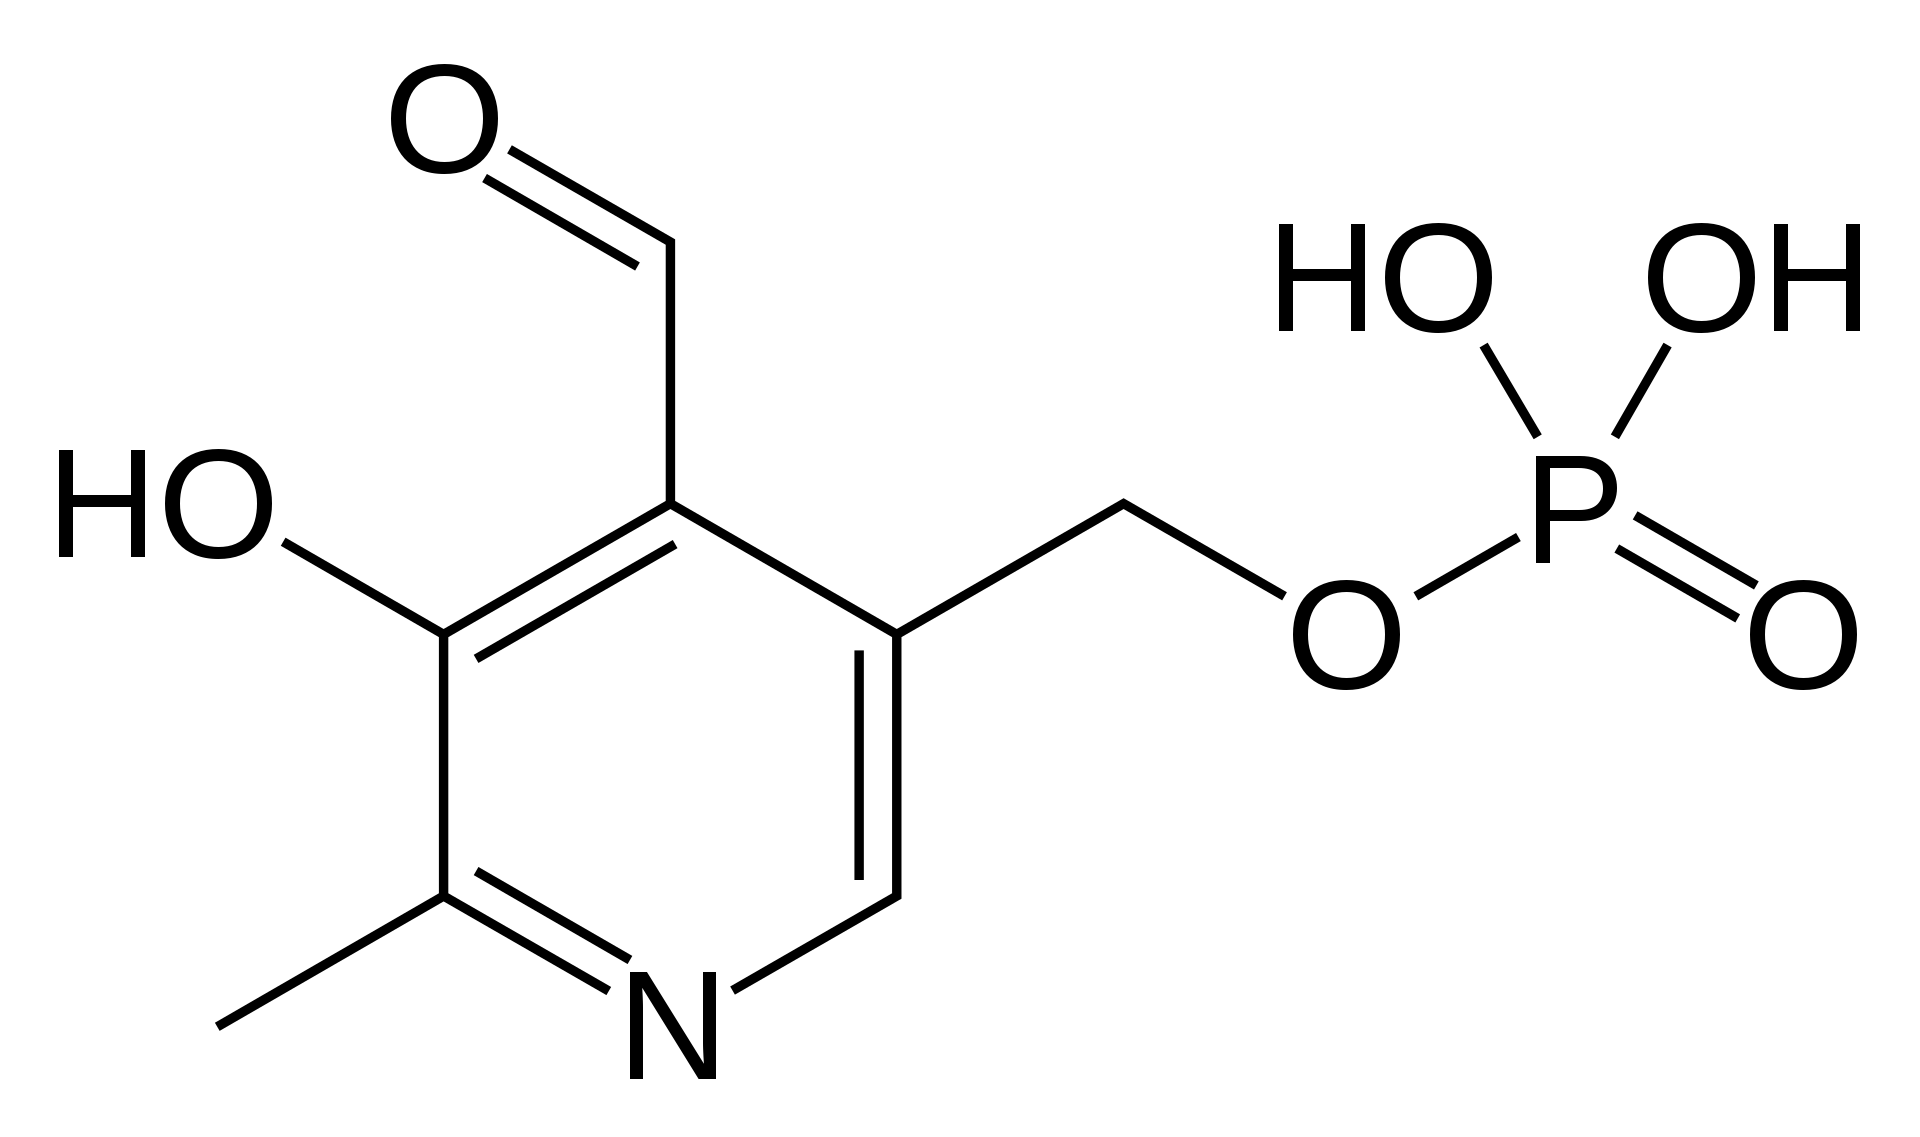
\includegraphics[width=0.75\linewidth]{images/Vitamin_B6_chemical_structure}
	\caption{Chemical structure of Vitamin B6}
\end{figure}

\section{About}


\section{Measurement unit}


\section{Dietary recommendations}


\section{Sources}


\chapter{Vitamin B7}
\begin{figure}[h]
	\centering 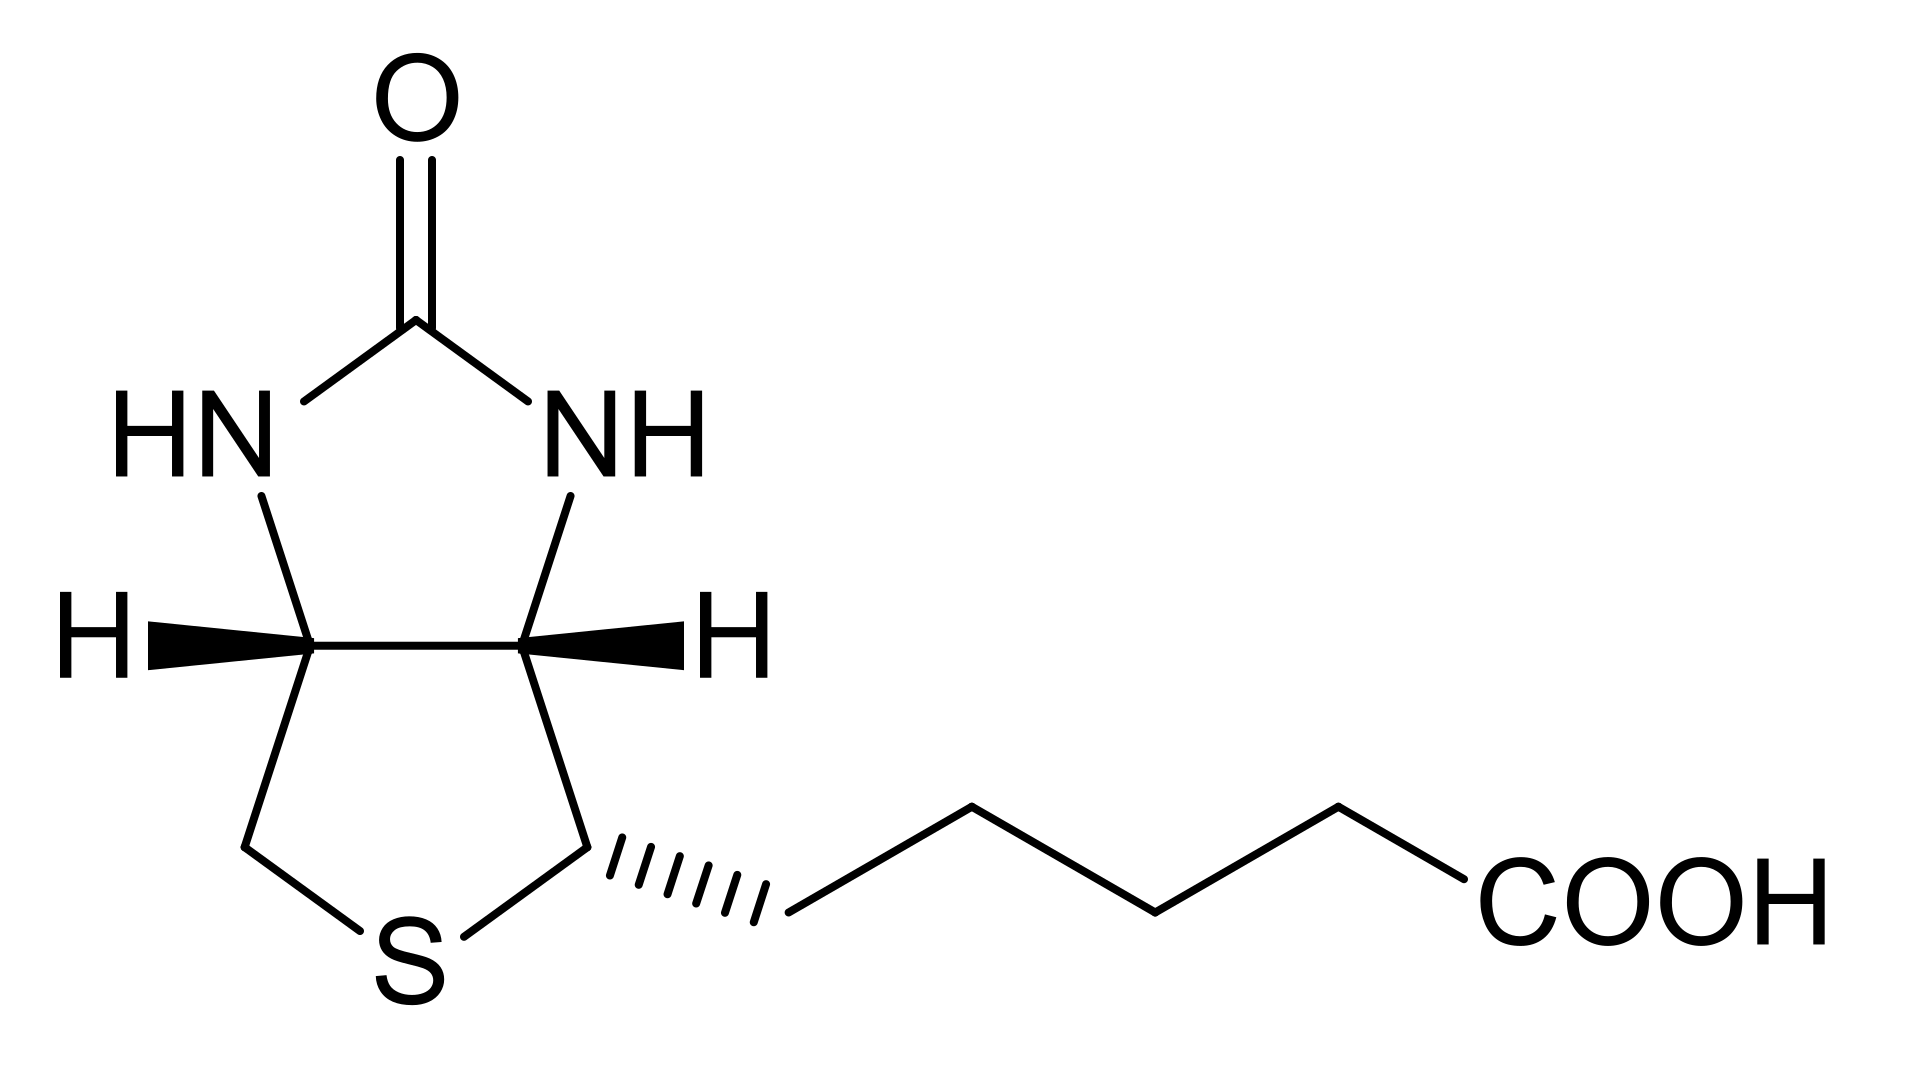
\includegraphics[width=0.75\linewidth]{images/Vitamin_B7_chemical_structure}
	\caption{Chemical structure of Vitamin B7}
\end{figure}

\section{About}


\section{Measurement unit}


\section{Dietary recommendations}


\section{Sources}


\chapter{Vitamin B9}
\begin{figure}[h]
	\centering 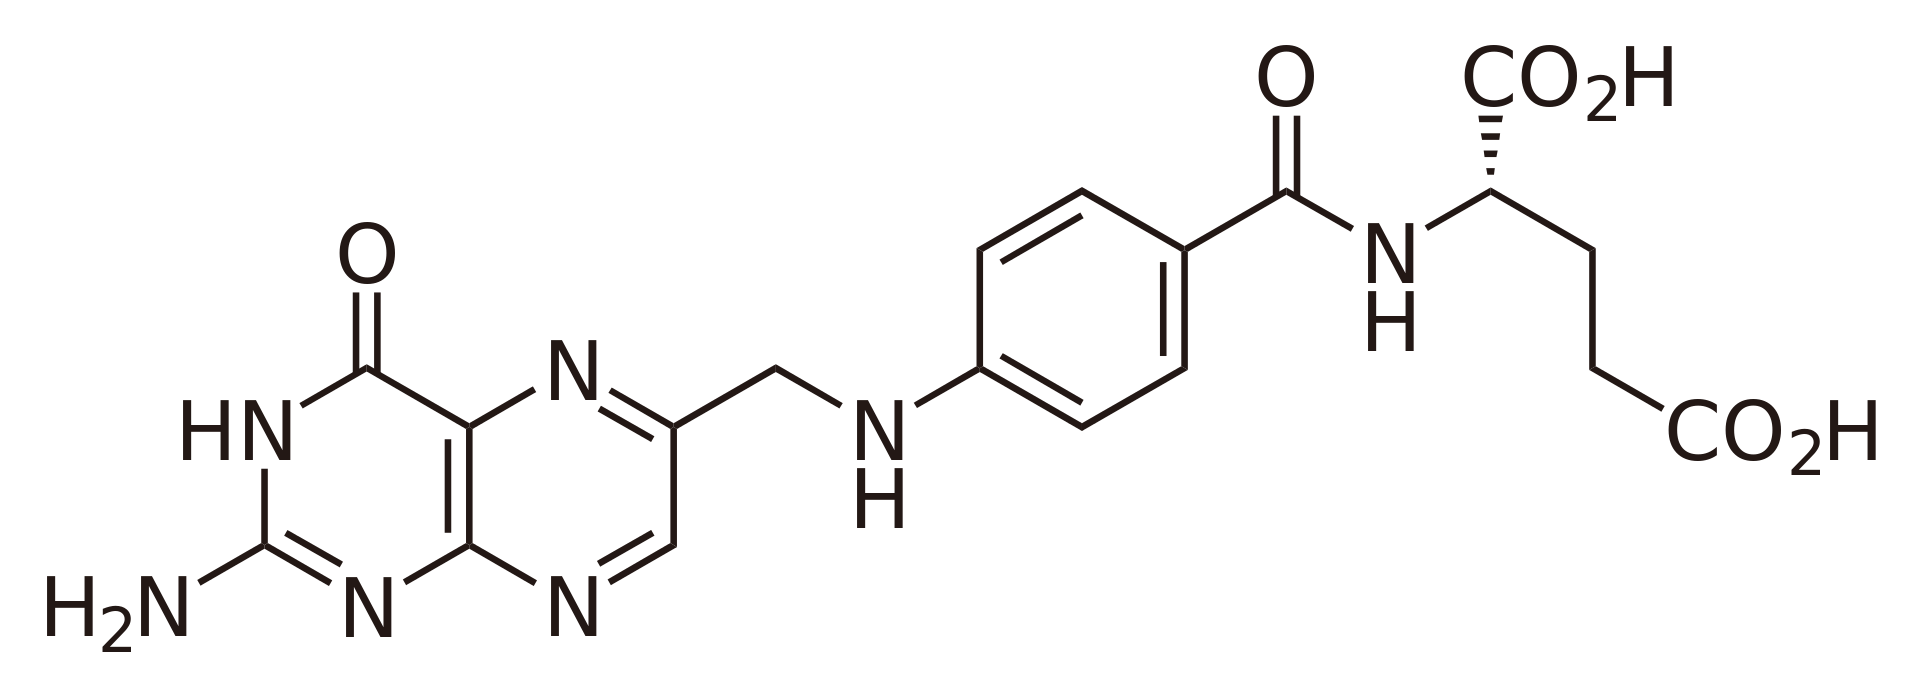
\includegraphics[width=0.75\linewidth]{images/Vitamin_B9_chemical_structure}
	\caption{Chemical structure of Vitamin B9}
\end{figure}

\section{About}


\section{Measurement unit}


\section{Dietary recommendations}


\section{Sources}


\chapter{Vitamin B12}
\begin{figure}[h]
	\centering 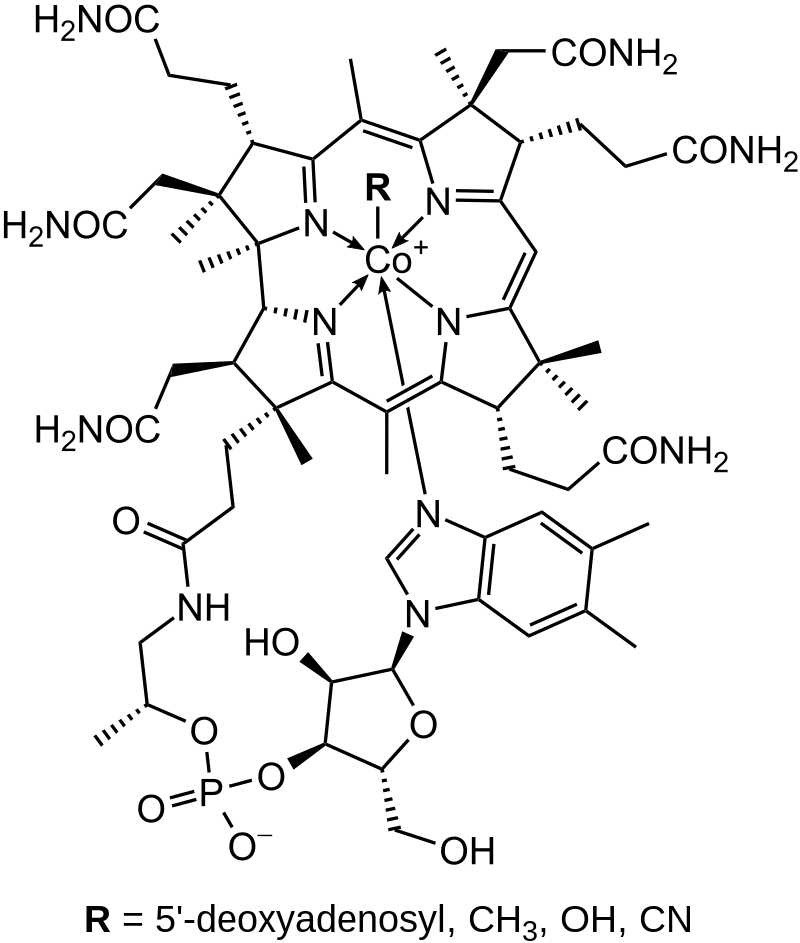
\includegraphics[width=0.75\linewidth]{images/Vitamin_B12_chemical_structure}
	\caption{Chemical structure of Vitamin B12}
\end{figure}

\section{About}


\section{Measurement unit}


\section{Dietary recommendations}


\section{Sources}


\chapter{Vitamin C}
\begin{figure}[h]
	\centering 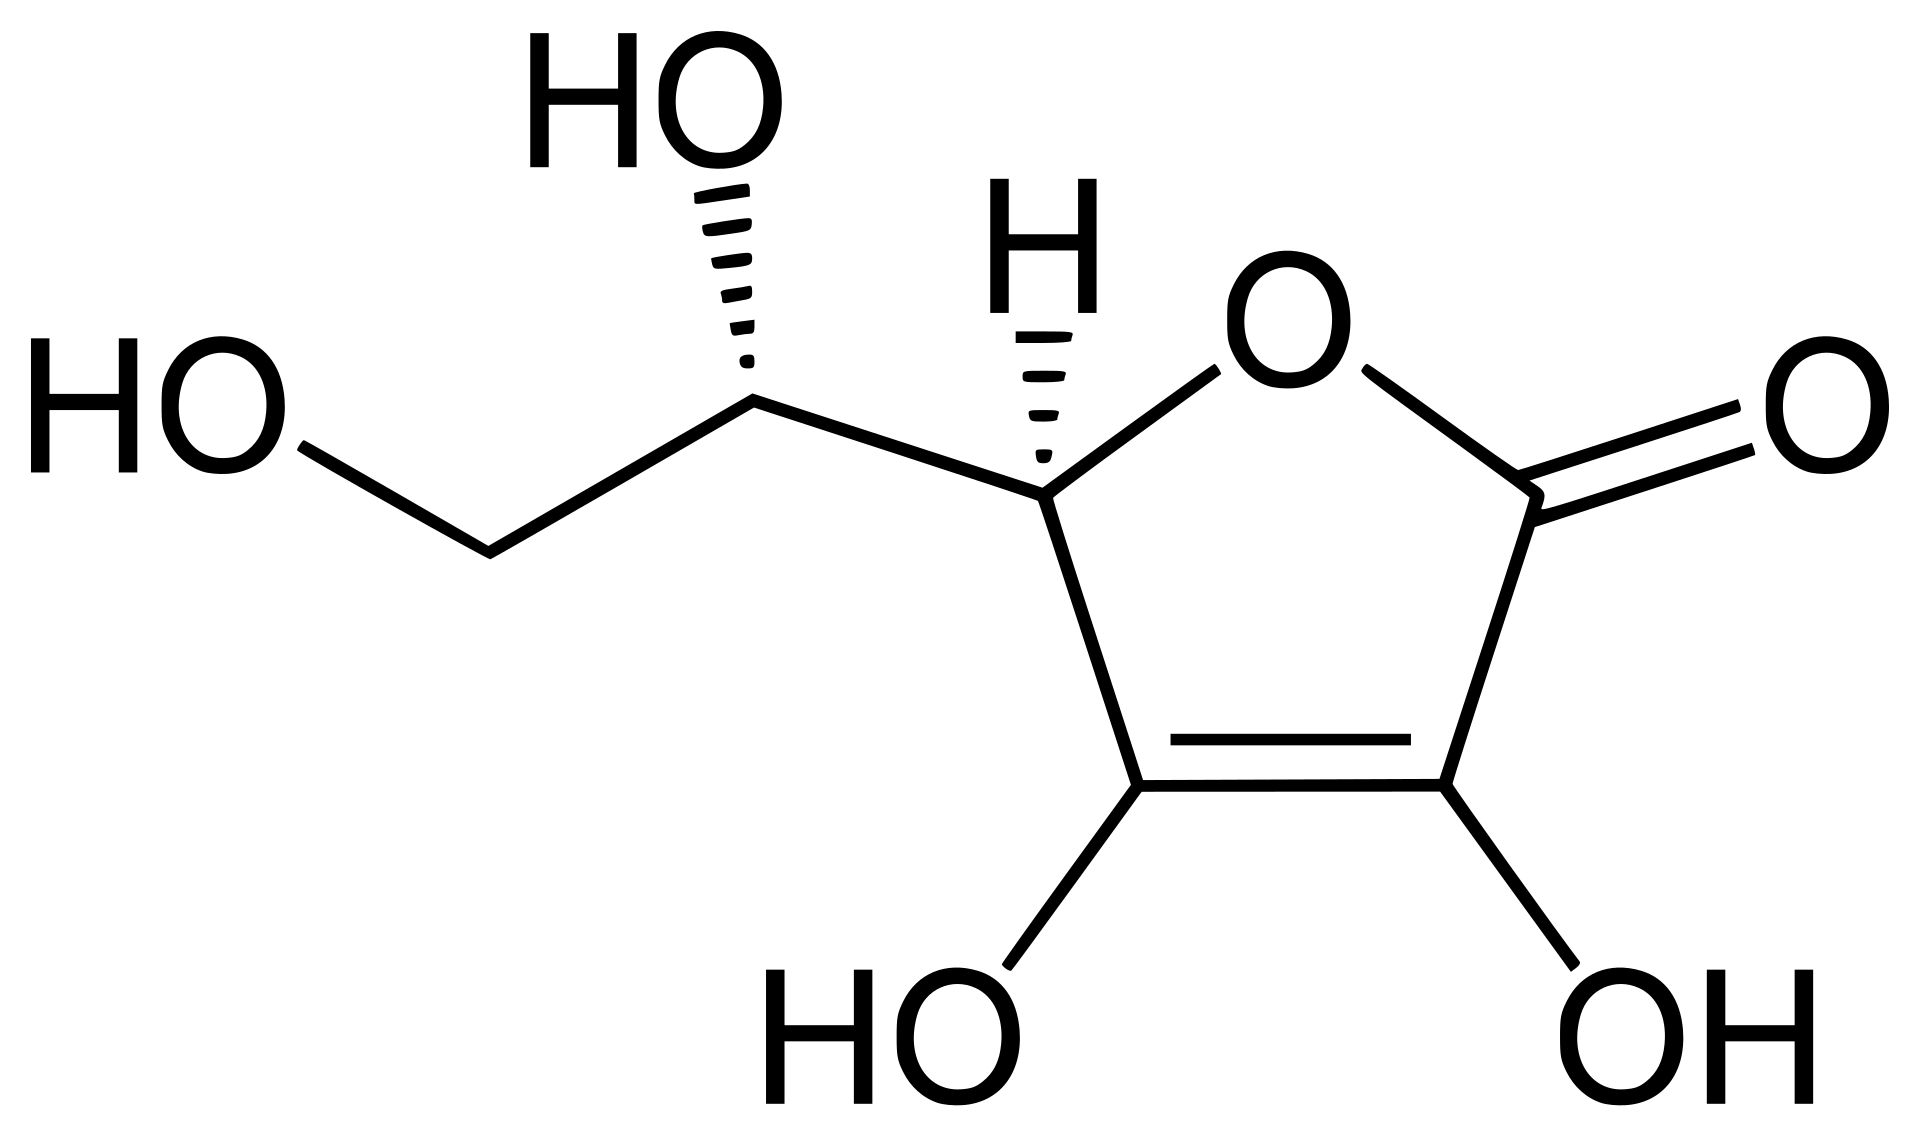
\includegraphics[width=0.75\linewidth]{images/Vitamin_C_chemical_structure}
	\caption{Chemical structure of Vitamin C}
\end{figure}

\section{About}


\section{Measurement unit}


\section{Dietary recommendations}


\section{Sources}


\chapter{Vitamin D}
\begin{figure}[h]
	\centering 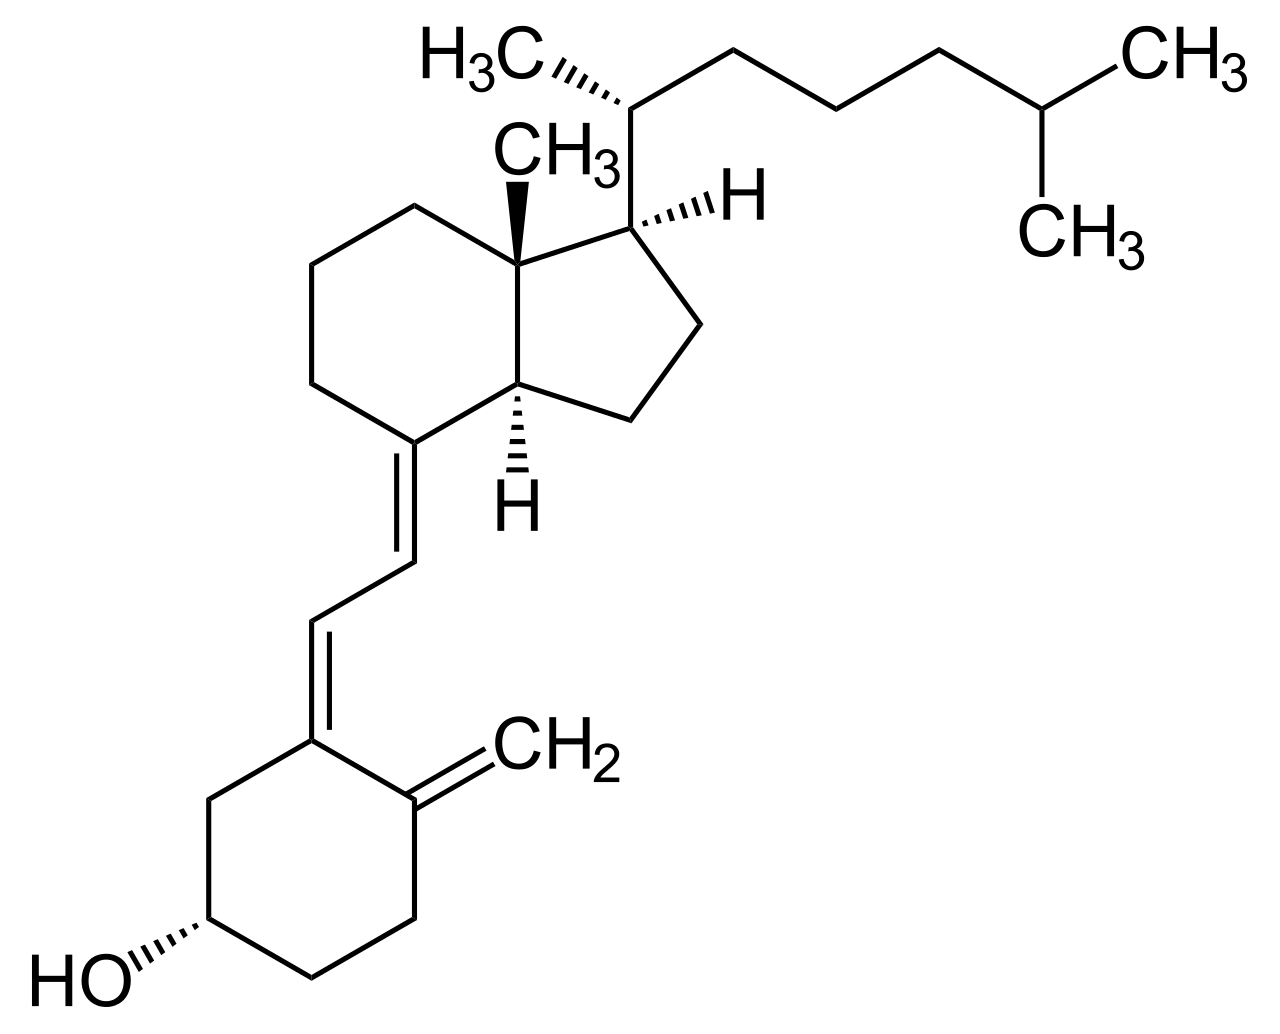
\includegraphics[width=0.75\linewidth]{images/Vitamin_D_chemical_structure}
	\caption{Chemical structure of Vitamin D}
\end{figure}

\section{About}


\section{Measurement unit}


\section{Dietary recommendations}


\section{Sources}


\chapter{Vitamin E}
\begin{figure}[h]
	\centering 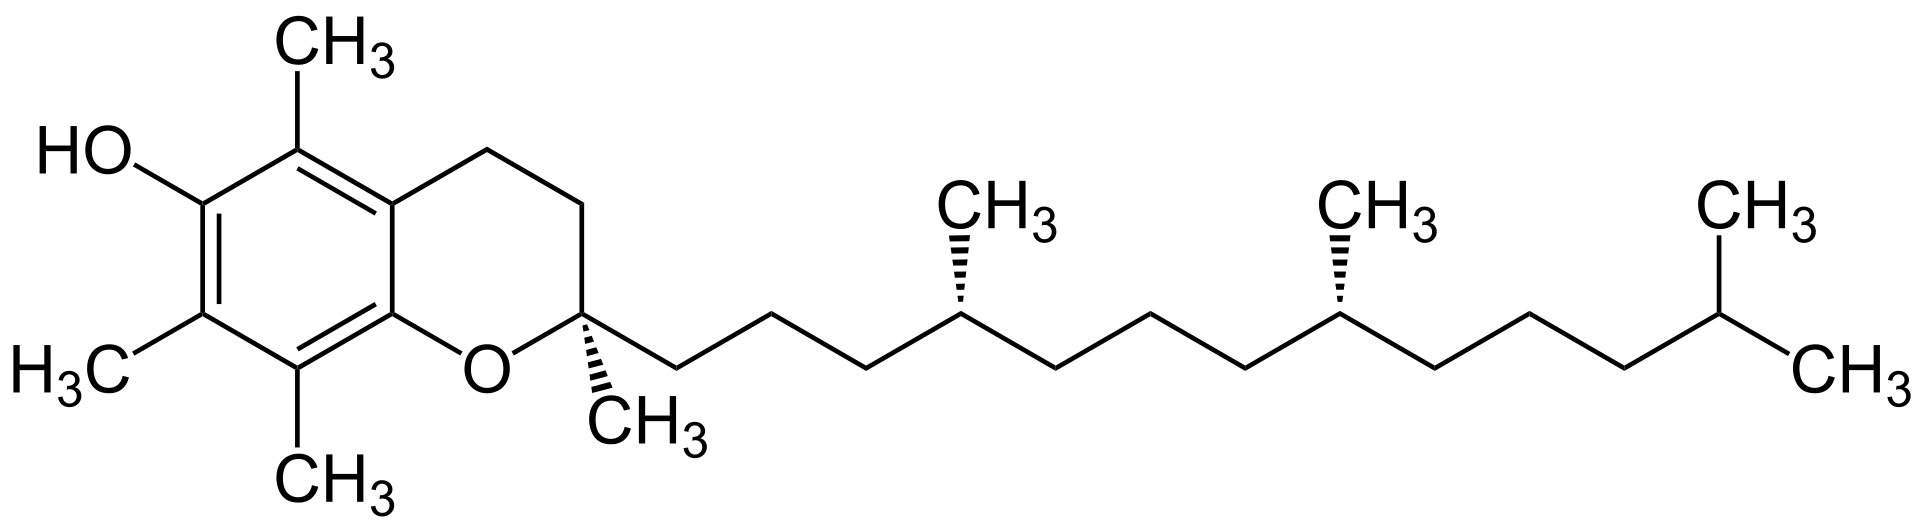
\includegraphics[width=0.75\linewidth]{images/Vitamin_E_chemical_structure}
	\caption{Chemical structure of Vitamin E}
\end{figure}

\section{About}


\section{Measurement unit}


\section{Dietary recommendations}


\section{Sources}


\chapter{Vitamin K1}
\begin{figure}[h]
	\centering 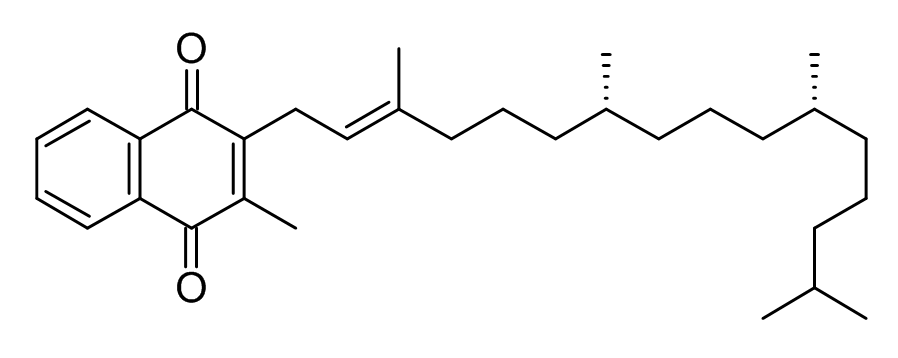
\includegraphics[width=0.75\linewidth]{images/Vitamin_K1_chemical_structure}
	\caption{Chemical structure of Vitamin K1}
\end{figure}

\section{About}


\section{Measurement unit}


\section{Dietary recommendations}


\section{Sources}


\chapter{Vitamin K2}
\begin{figure}[h]
	\centering 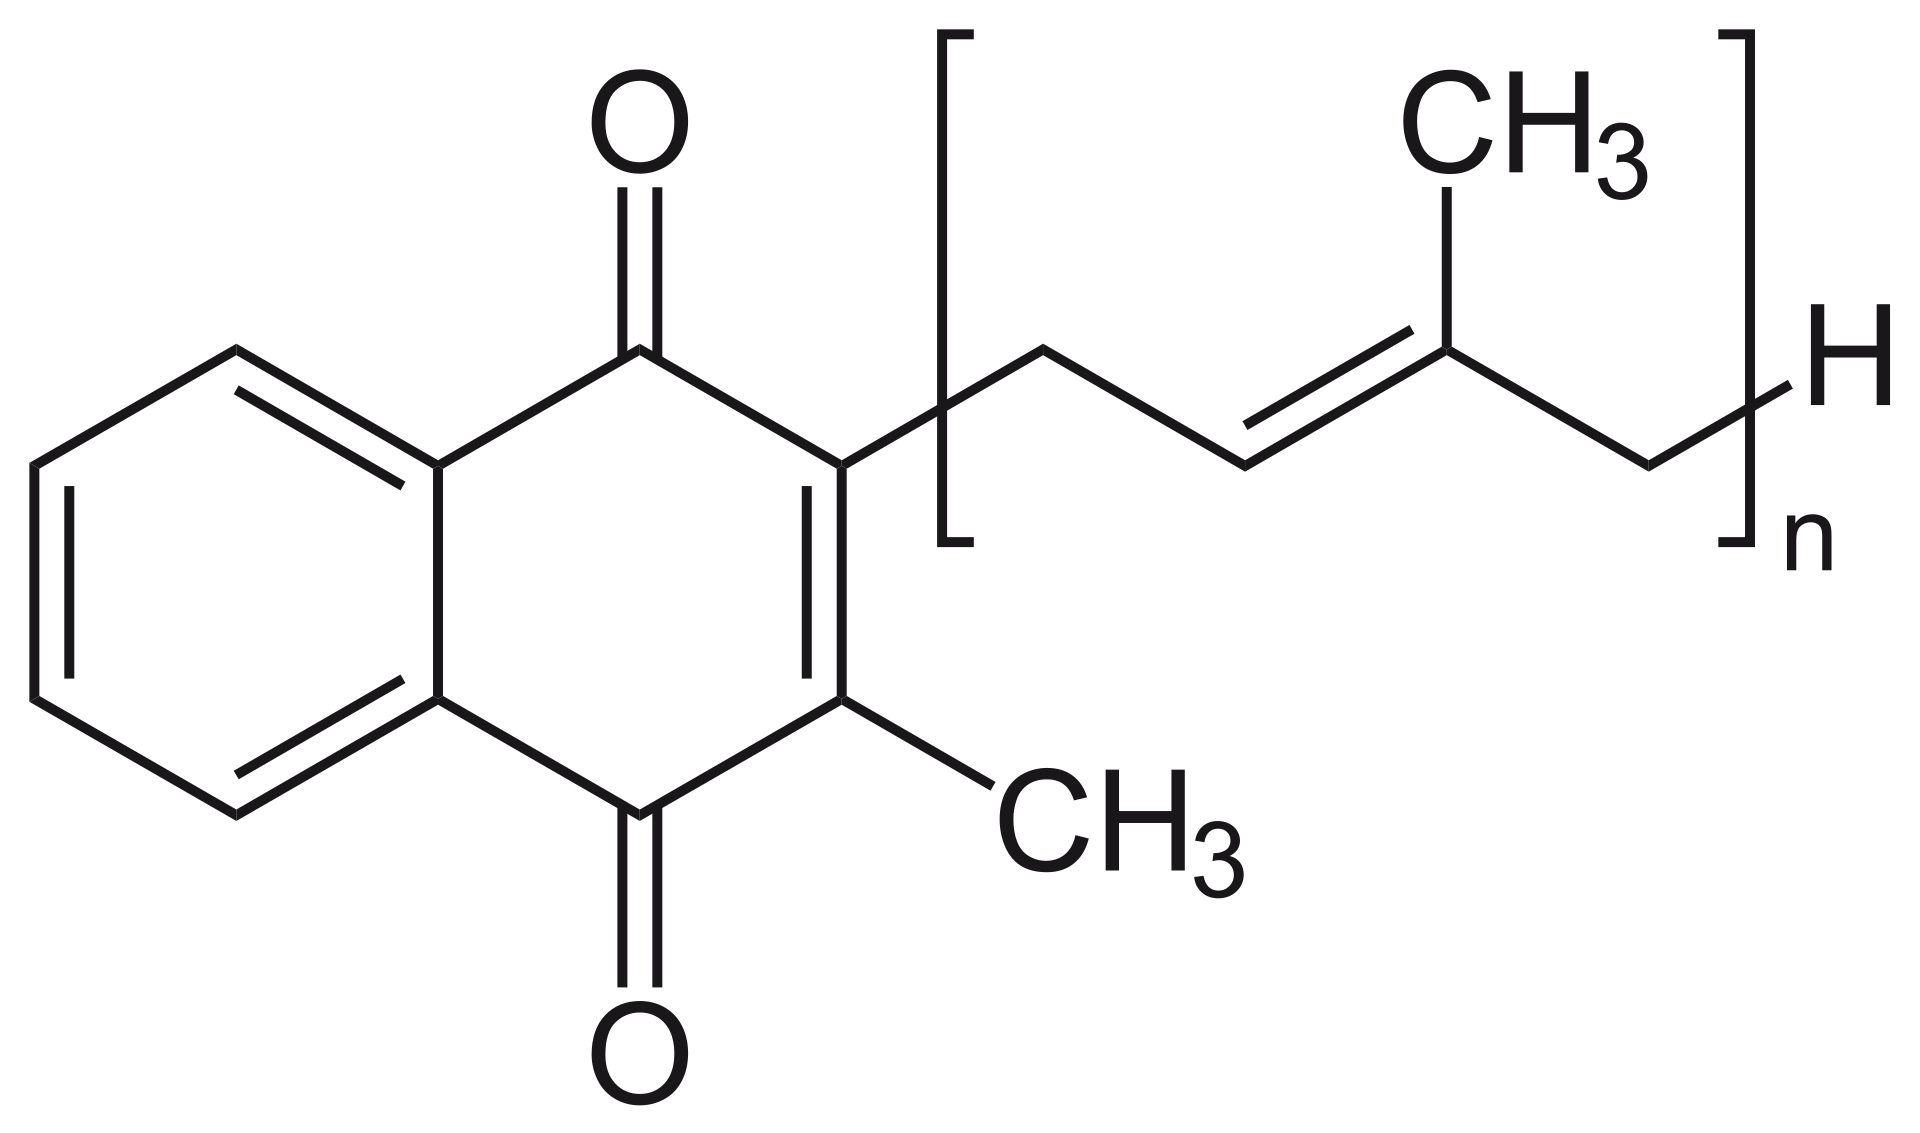
\includegraphics[width=0.75\linewidth]{images/Vitamin_K2_chemical_structure}
	\caption{Chemical structure of Vitamin K2}
\end{figure}

\section{About}


\section{Measurement unit}


\section{Dietary recommendations}


\section{Sources}


\chapter{Vitamin K3}
\begin{figure}[h]
	\centering 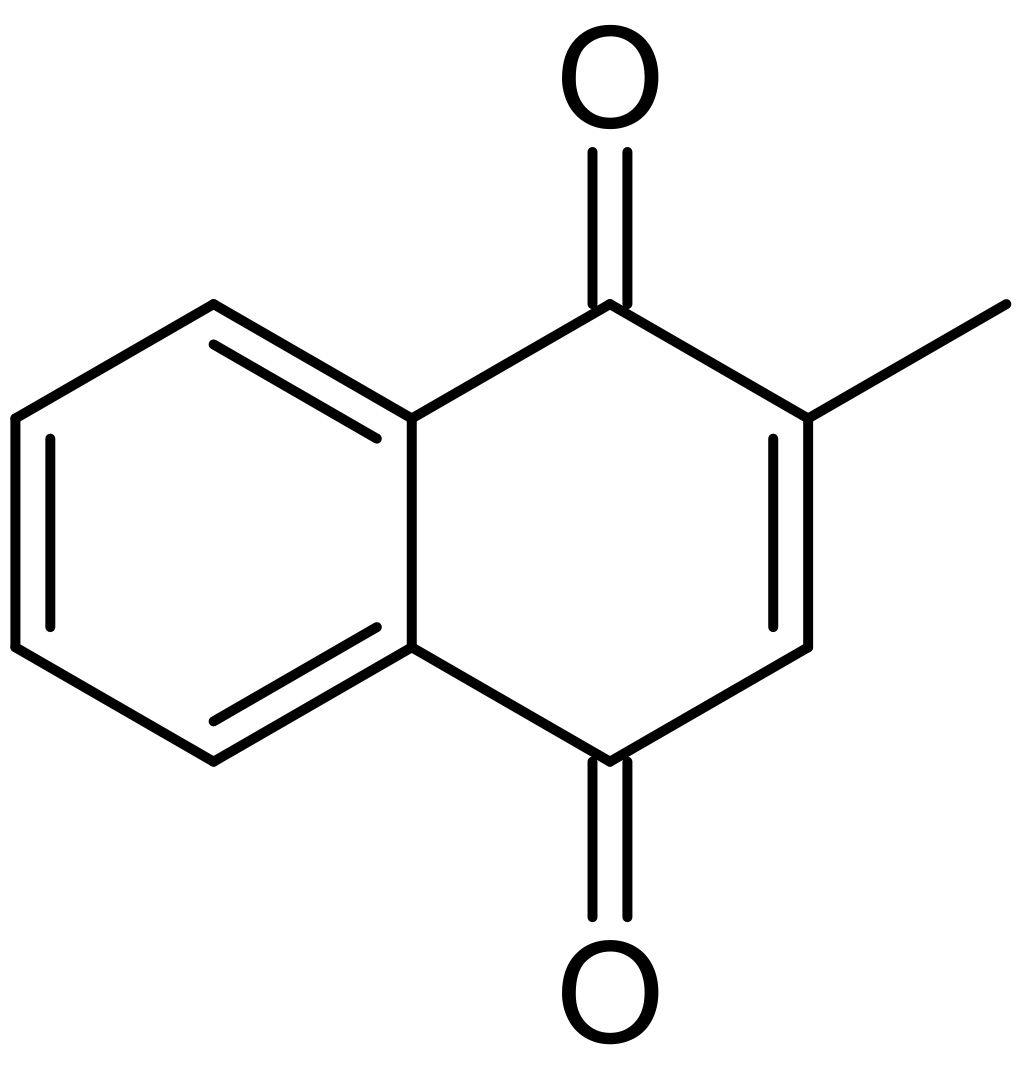
\includegraphics[width=0.75\linewidth]{images/Vitamin_K3_chemical_structure}
	\caption{Chemical structure of Vitamin K3}
\end{figure}

\section{About}


\section{Measurement unit}


\section{Dietary recommendations}


\section{Sources}


\chapter{Choline}
\begin{figure}[h]
	\centering 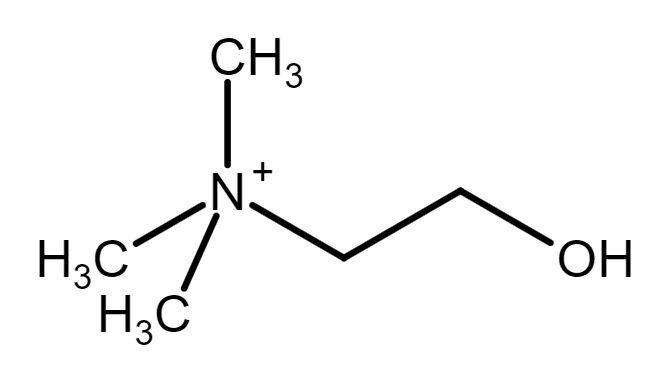
\includegraphics[width=0.75\linewidth]{images/Choline_chemical_structure}
	\caption{Chemical structure of Choline}
\end{figure}

\section{About}


\section{Measurement unit}


\section{Dietary recommendations}


\section{Sources}


\listoffigures
\listoftables

\end{document}